
\chapter{Formule di Logica modale e significato}

$a$ è vera nel mondo $\alpha$, e scriviamo $\mu\models_{\alpha}a$

se 
\begin{itemize}
\item $a$ è una lettera enunciativa allora deve valere $\verita a{\alpha}$ 
\item $a$ è del tipo: $a\lor b$ .... allora.... $\mu\models_{\alpha}a$
oppure $\mu\models_{\alpha}b$ 
\end{itemize}

\section{Relazione seriale}

Ip) Frame F con relazione R seriale

Ts) $\boa\implies\dia$

Dimostrazione:

Se non vale: $\veraw{\mu}{\alpha}{\boa}$ allora immediatemente si
ha la tesi in quanto l'antecedente è falso.

Se invce: $\veraw{\mu}{\alpha}{\boa}$ allora

$\forhten{\beta}{\,:\,\alpha R\beta}{\veraw{\mu}{\beta}a}$ per definizione
di box,

inoltre dato che R seriale per Ip si ha anche che $\exists\beta:\:(\alpha,\beta)\:\in R$

da cui: $\veraw{\mu}{\alpha}{\dia}$ per definizione di diamond (esiste
$\beta$ in relazione con $\alpha$ per la serialità e in $\alpha$
vale $a$ dato che $\veraw{\mu}{\alpha}{\boa}$ )\\


Ip) $\boa\implies\dia$

Ts) Frame F con relazione R seriale

\begin{center}
$ $\begin{center}  
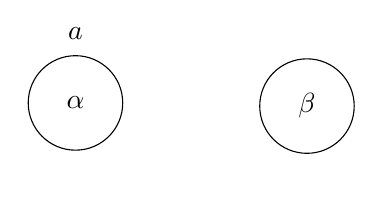
\begin{tikzpicture}[scale=0.2]  
\tikzstyle{every node}+=[inner sep=0pt]  
\draw [black] (24.2,-13) circle (3); 
\draw (24.2,-13) node {$\alpha$};
\draw (24.2,-8.6) node {$\boxx{a}$};
\draw [black] (38.9,-13.2) circle (3);
\draw (38.9,-13.2) node {$\beta$}; 
\draw (24,-17.3) node {\sout{$\dia$}};   
\end{tikzpicture} \end{center}
\par\end{center}

Per assurdo:

Suppongo di trovarmi in un mondo come quello in figura (wow) in cui
\mbox{$\veraw{\mu}{\alpha}{\boa}$ }, e suppongo che la relazione
R del frame NON sia seriale cioè $\sim\exists\beta:(\alpha R\beta)$,
se è così vale sicuramente $\veraw{\mu}a{\boa}$ (dato che $\alpha$
non ha successori) , d'altra parte per come è il mondo considerato,
cioè si nega la tesi, assurdo\sout{.}


\section{Relazione riflessiva}

Ip) R riflessiva

Ts) $\boa\implies a$

se l'antecedente è falso il teorema è dimostrato, consideriamo il
caso in cui l'antecedente è vero:

$\veraw{\mu}{\alpha}{\boa}$

poichè il frame è riflessivo, abbiamo $\alpha R\alpha$, e quindi
varrà:

$\veraw{\mu}{\alpha}a$

e la tesi è dimostrata.

\begin{center} 
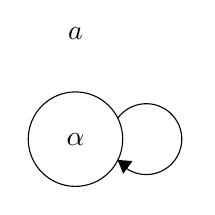
\begin{tikzpicture}[scale=0.2] 
\tikzstyle{every node}+=[inner sep=0pt] 
\draw [black] (32.4,-24.8) circle (3); 
\draw (32.4,-24.8) node {$\alpha$}; 
\draw (32.4,-20.6) node {$\boa$}; 
\draw (32.4,-18.1) node {$a$}; 
\draw [black] (35.08,-23.477) arc (144:-144:2.25); 
\fill [black] (35.08,-26.12) -- (35.43,-27) -- (36.02,-26.19); 
\end{tikzpicture} \end{center}

Ip) $\boa\implies a$

Ts) R è riflessiva

Supponiamo per assurdo che R non sia riflessiva, allora prendiamo
uno stato $\alpha$ tale che $\nexists\beta:\,\alpha R\beta$. Allora
si avrà che:

$\veraw{\mu}{\alpha}{\boa}\wedge\nonveraw{\mu}{\alpha}a$

che è assurdo perchè contraddice la tesi. La tesi allora è valida.

\begin{center} 
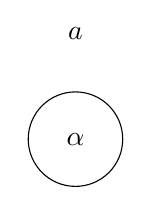
\begin{tikzpicture}[scale=0.2] 
\tikzstyle{every node}+=[inner sep=0pt] 
\draw [black] (32.4,-24.8) circle (3); 
\draw (32.4,-24.8) node {$\alpha$}; 
\draw (32.4,-20.6) node {$\boa$}; 
\draw (32.4,-18.1) node {\sout{$a$}}; 
\end{tikzpicture} 
\end{center}


\section{Relazione simmetrica}

Ip) R simmetrica

Ts) $a\implies\boxx{\dia}$

Suppongo che $\veraw{\mu}{\alpha}a$ (se no avrei già la tesi), due
casi:

\textbf{Caso 1}: Da $\alpha$ non parte nessun arco, allora sicuramente
$\veraw{\mu}{\alpha}{\boxx x}$ con $x$ qualsiasi e in particolare
$\veraw{\mu}{\alpha}{\boxx{\dia}}$

\begin{center}
\begin{center} 
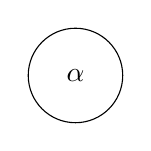
\begin{tikzpicture}[scale=0.2] 
\tikzstyle{every node}+=[inner sep=0pt] 
\draw [black] (24.2,-13) circle (3);
\draw (24.2,-13) node {$\alpha$};
\end{tikzpicture}
\end{center} 
\par\end{center}

\textbf{Caso 2}: Esiste almeno un $\beta$ tale che $\alpha R\beta$.

\begin{center}
\begin{center} 
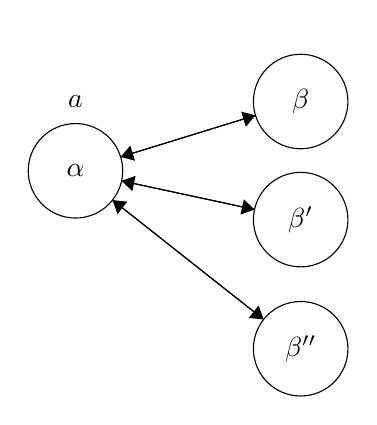
\begin{tikzpicture}[scale=0.2] 
\tikzstyle{every node}+=[inner sep=0pt] 
\draw [black] (24.2,-12.7) circle (3); 
\draw (24.2,-12.7) node {$\alpha$};
\draw (24.2,-8.3) node {$a$};  
\draw [black] (38.5,-8.3) circle (3);
 \draw (38.5,-8.3) node {$\beta$}; 
\draw [black] (38.5,-15.8) circle (3);  
\draw (38.5,-15.8) node {$\beta'$};  
\draw [black] (38.5,-24) circle (3);  
\draw (38.5,-24) node {$\beta''$}; 
\draw (38.5,-3.7) node {$\dia$};
\draw (38.5,-11.7) node {$\dia$};  \draw (38.5,-20.2) node {$\dia$}; 
\draw [black] (27.07,-11.82) -- (35.63,-9.18); \fill [black] (35.63,-9.18) -- (34.72,-8.94) -- (35.02,-9.9);  \draw [black] (35.63,-9.18) -- (27.07,-11.82);  \fill [black] (27.07,-11.82) -- (27.98,-12.06) -- (27.68,-11.1); \draw [black] (27.13,-13.34) -- (35.57,-15.16); \fill [black] (35.57,-15.16) -- (34.89,-14.51) -- (34.68,-15.48); \draw [black] (35.57,-15.16) -- (27.13,-13.34);  \fill [black] (27.13,-13.34) -- (27.81,-13.99) -- (28.02,-13.02);  \draw [black] (26.55,-14.56) -- (36.15,-22.14); \fill [black] (36.15,-22.14) -- (35.83,-21.25) -- (35.21,-22.04);  \draw [black] (36.15,-22.14) -- (26.55,-14.56);  \fill [black] (26.55,-14.56) -- (26.87,-15.45) -- (27.49,-14.66); \end{tikzpicture} \end{center}
\par\end{center}

Dato che la relazione è simmetrica se $\alpha R\beta$ allora \textbf{$\beta R\alpha$.}
Dato che $\veraw{\mu}{\alpha}a,$ in ognuno di questi $\beta$, $\beta'$,$\beta''$
ecc. vale $\dia$ perché ognuno di loro è in relazione con $\alpha$.

Allora per ognuno di questi $\beta$ si ha $\veraw{\mu}{\beta}{\dia}$,
(esiste infatti un mondo, $\alpha$, in cui vale $a$) da cui: $\veraw{\mu}{\alpha}{\boxx{\dia}}$
\\


Ip) $a\implies\boxx{\dia}$

Ts) R simmetrica

Per assurdo:

suppongo R non sia simmetrica e considero un frame con soli $\alpha$
e $\beta$ e in cui $R=\{(\alpha,\beta)\}$ . In questo frame considero
un modello con funzione di verità tale che: $V(A)=\{\alpha\}$.

In $\beta$ non vale $\dia$ perché $\beta$ non è in relazione con
nessun mondo, per questo: $\nonveraw{\mu}{\alpha}{\boxx{\dia}}$

\begin{center}
\begin{center}  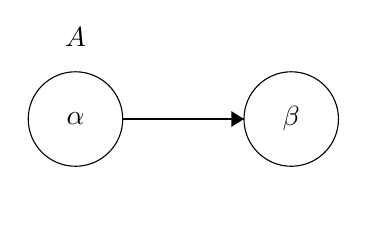
\begin{tikzpicture}[scale=0.2] \tikzstyle{every node}+=[inner sep=0pt]  \draw [black] (24.2,-12.7) circle (3);  \draw (24.2,-12.7) node {$\alpha$}; 
\draw (24.2,-7.5) node {$A$};
\draw [black] (37.9,-12.7) circle (3); \draw (37.9,-12.7) node {$\beta$};
\draw (37.9,-7.5) node {\sout{$\dia$}}; 
\draw (24.2,-17.8) node {\sout{$\boxx{\dia}$}}; 
\draw [black] (27.2,-12.7) -- (34.9,-12.7); \fill [black] (34.9,-12.7) -- (34.1,-12.2) -- (34.1,-13.2);  \end{tikzpicture} \end{center}
\par\end{center}

$ $


\section{Relazione Transitiva}

Ip) R relazione transitiva

Ts) $\boa\implies\boxx{\boa}$

Se $\nonveraw{\mu}{\alpha}{\boa}$ la tesi è dimostrata, consideriamo
allora il caso in cui $\veraw{\mu}{\alpha}{\boa}$

per ipotesi:

$\exists\beta\,:\,(\alpha,\beta)\,\in R\,(\beta,\gamma)\,\in R$

allora abbiamo che:

$(\alpha,\gamma)\,\in R$

$\veraw{\mu}{\gamma}a$ 

e quindi varrà ovviamente che:

$\veraw{\mu}{\beta}a$

da cui segue:

$\veraw{\mu}{\alpha}{\boxx{\boa}}$ 

e la tesi è dimostrata.

\begin{center} \begin{tikzpicture}[scale=0.2] 
\tikzstyle{every node}+=[inner sep=0pt] 
\draw [black] (16,-26.5) circle (3); 
\draw (16,-26.5) node {$\alpha$}; 
\draw [black] (36.8,-16.1) circle (3); 
\draw (36.8,-16.1) node {$\beta_1$}; 
\draw [black] (54.2,-25.4) circle (3); 
\draw (54.2,-25.4) node {$\gamma$}; 
\draw [black] (37.5,-38.1) circle (3); 
\draw (37.5,-38.1) node {$\beta_2$}; 
\draw (15.9,-21.5) node {$\boa$}; 
\draw (37.5,-33.4) node {$\boa$}; 
\draw (15.9,-18) node {$\boxx{\boa}$}; 
\draw (36.8,-11.9) node {$\boa$}; 
\draw (53.6,-20.6) node {$a$}; 
\draw [black] (18.68,-25.16) -- (34.12,-17.44); 
\fill [black] (34.12,-17.44) -- (33.18,-17.35) -- (33.62,-18.25); 
\draw [black] (39.45,-17.51) -- (51.55,-23.99); \fill [black] (51.55,-23.99) -- (51.08,-23.17) -- (50.61,-24.05); 
\draw [black] (19,-26.41) -- (51.2,-25.49); \fill [black] (51.2,-25.49) -- (50.39,-25.01) -- (50.42,-26.01); 
\draw [black] (18.64,-27.92) -- (34.86,-36.68); 
\fill [black] (34.86,-36.68) -- (34.39,-35.86) -- (33.92,-36.74); 
\end{tikzpicture} 
\end{center}

Ip) $\boa\implies\boxx{\boa}$

Ts) R relazione transitiva

supponiamo per assurdo che esista uno stato$\alpha$ per cui non vale
la proprietà transitiva

consideriamo il caso in cui valga la seguente funzione di valutazione:

$V(a)=\{S\,|\,(\alpha,\delta)\,\in R\}$ 

Allora a sarà vera in $\beta$, ma non in $\gamma$. per cui in $\alpha$
sarà vera $\boa$ ma non $\boxx{\boa}$

\begin{center} 
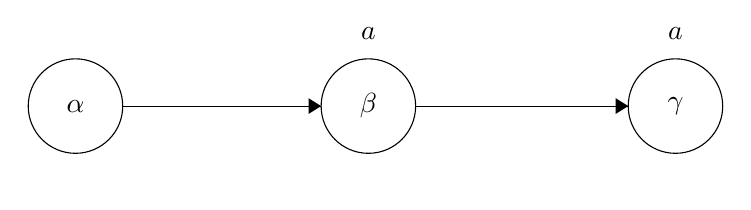
\begin{tikzpicture}[scale=0.2] \tikzstyle{every node}+=[inner sep=0pt] 
\draw [black] (16,-28.2) circle (3); 
\draw (16,-28.2) node {$\alpha$}; 
\draw [black] (34.6,-28.2) circle (3); 
\draw (34.6,-28.2) node {$\beta$}; 
\draw [black] (54.1,-28.2) circle (3); 
\draw (54.1,-28.2) node {$\gamma$}; 
\draw (16,-23.6) node {$\boa$}; 
\draw (34.6,-23.6) node {$a$}; 
\draw (54.1,-23.6) node {\sout{$a$}}; 
\draw (16,-32.9) node {\sout{$\boxx{\boa}$}}; 
\draw (34.6,-32.9) node {\sout{$\boa$}}; 
\draw [black] (19,-28.2) -- (31.6,-28.2); 
\fill [black] (31.6,-28.2) -- (30.8,-27.7) -- (30.8,-28.7); 
\draw [black] (37.6,-28.2) -- (51.1,-28.2); 
\fill [black] (51.1,-28.2) -- (50.3,-27.7) -- (50.3,-28.7); 
\end{tikzpicture} 
\end{center}




\section{Funzione parziale}

\begin{tabular}{|c|c|c|}
\hline 
$\diam a\implies\boxx a$  & funzione parziale  & $\forhten{\alpha}{:\,\alpha R\beta,\:\beta R\gamma}{\beta}=\gamma$\tabularnewline
\hline 
\end{tabular}

Funzione parziale, dimostrazione

.

Ip) funzione parziale

Ts) $\diam a\implies\boxx a$ 

.

$\diam{}a$ falsa allora dato che l'antecedente è falso di ha $\implica{\diam{}a}{\boxx a}$

$\diam{}a$ vera allora $\exists\beta$:$\alpha R\beta$ e$\in V(\beta)$,
ma dato che la funzione è parziale questo $\beta$ è unico !

da cui $\vera{\mu}{\implica{\diamond a}{\boxx a}}$

.

.

Ip) $\diam a\implies\boxx a$ 

Ts) funzione parziale

.

.

Per assurdo: suppongo non che la funzione non sia parziale. Se è così
$\exists\alpha:$ $\alpha R\beta,$ $\alpha R\gamma$, considero un
modello in cui V(A) = \{$\beta$ \} , $\boxx A$ non vale in $\alpha$
dato che A è falsa in $\gamma$, il che contraddice l'ipotesi (BAM!)\\
 \\
 


\section{Funzione totale}

\begin{tabular}{|c|c|c|}
\hline 
$\dia\iff\boxx a$  & funzione totale  & $\forall\alpha\exists\,!\,\beta:\:\alpha R\beta$ \tabularnewline
\hline 
\end{tabular}\\
 \\


non ci sono ``conti'' da fare, R è seriale sse R è seriale $\boxx a\implies\diam a$
, e se R è una funzione parziale $\implica{\diam a}{\boxx a}$

quindi dato che l'implica prevede un and di implica da una parte e
dall'altra per definizione abbiamo la tesi

.


\section{Relazione euclidea}

\begin{tabular}{|c|c|c|}
\hline 
$\dia\implies\boxx{\diam a}$  & relazione euclidea  & $\forhten{\alpha,\beta,\gamma}{:\:(\alpha R\beta,\:\alpha R\gamma)}{\beta}R\gamma$
da cui anche: $\beta$R$\beta$, $\gamma R\gamma$, $\gamma$R$\beta$\tabularnewline
\hline 
\end{tabular}\\
 \\


Ip) relazione euclidea

Ts) $\diam a\implies\boxx{\diam a}$

Suppongo sia vero l'antecedente (se falso ho finito), quindi vale:
$\dia$ da cui: $\vera{\mu}{\dia}$

dato che $\dia$ si ha che esiste almeno un $\beta$ tale che in beta
vale a

solo un beta: autoanello perché euclidea e quindi $\boxx{\dia}$

diversi beta: ognuno dei vari $\beta'$, $\beta''$ , ecc. sono in
relazione con $\beta$, dato che la relazione è euclidea, pertanto
dato che in $\beta$ vale $a$, in ognuno di loro vale $\dia$ \\


\begin{center}
 \begin{center}  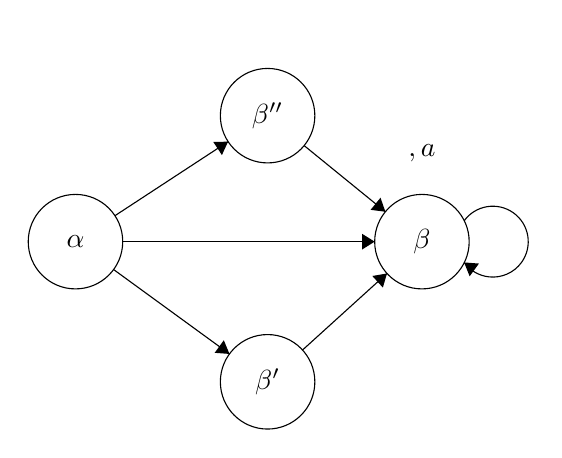
\begin{tikzpicture}[scale=0.2]  \tikzstyle{every node}+=[inner sep=0pt] \draw [black] (24.5,-18.4) circle (3); \draw (24.5,-18.4) node {$\alpha$}; \draw [black] (46.5,-18.4) circle (3);  \draw (46.5,-18.4) node {$\beta$}; \draw [black] (36.7,-27.3) circle (3);  \draw (36.7,-27.3) node {$\beta'$}; \draw (23.9,-12.8) node {$\dia$}; \draw (46.5,-12.8) node {$\dia, a$}; \draw (36.7,-22.1) node {$\dia$}; \draw [black] (36.7,-10.4) circle (3); \draw (36.7,-10.4) node {$\beta''$}; \draw (36.7,-4.9) node {$\dia$}; \draw [black] (27.5,-18.4) -- (43.5,-18.4);  \fill [black] (43.5,-18.4) -- (42.7,-17.9) -- (42.7,-18.9); \draw [black] (26.92,-20.17) -- (34.28,-25.53);  \fill [black] (34.28,-25.53) -- (33.92,-24.66) -- (33.34,-25.46);  \draw [black] (27.01,-16.75) -- (34.19,-12.05);  \fill [black] (34.19,-12.05) -- (33.25,-12.07) -- (33.8,-12.9);  \draw [black] (49.18,-17.077) arc (144:-144:2.25); \fill [black] (49.18,-19.72) -- (49.53,-20.6) -- (50.12,-19.79); \draw [black] (39.02,-12.3) -- (44.18,-16.5); \fill [black] (44.18,-16.5) -- (43.87,-15.61) -- (43.24,-16.38); \draw [black] (38.92,-25.28) -- (44.28,-20.42); \fill [black] (44.28,-20.42) -- (43.35,-20.58) -- (44.02,-21.32);  \end{tikzpicture} \end{center} 
\par\end{center}

Ip)$\dia\implies\boxx{\diam a}$

Ts) relazione euclidea

Per assurdo, suppondo valga ip) ma non la tesi

Considero un Frame in cui: $\alpha R\beta,$ $\alpha R\gamma,$ $\beta R\gamma$
ma NON $\beta R\gamma$ cioè si ha un frammento in cui non vale l'euclidea.
Poniamo che il modello sia tale che $V(A)$$=\{\gamma\}$

In queste ipotesi vale $\dia$ dato che in $\gamma$ vale $a$. In
$\beta$ non vale $a$ e neppure $\dia$ perché non ha ``uscite'',
da cui in $a$ non vale $\boxx{\dia}$ contraddicendo così l'ipotesi
(BAM!) 


\section{Relazione Debolmente Densa}

\begin{tabular}{|c|c|c|}
\hline 
$\dia\implies\diam{\diam a}$  & relazione debolmente densa  & $\forhten{\alpha,\beta}{:\:(\alpha R\beta)}{\exists\gamma:\,(\alpha R\gamma\wedge\gamma R\beta)}$\tabularnewline
\hline 
\end{tabular}

Ip) R debolmente densa

Ts) $\dia\implies\diam{\diam a}$ 

supponiamo che sia vero l'antecedente (se è falso la tesi è dimostrata)
avremo quindi:

$\veraw{\mu}{\alpha}{\dia}$

allora segue che:

$\exists\beta:\,\veraw{\mu}{\beta}a$

ma poichè la relazione è debolmente densa, si avrà che:

$\exists\gamma:\,(\alpha R\gamma\wedge\gamma R\beta)$

poichè in $\beta$ è vera a, allora segue:

$\veraw{\mu}{\gamma}{\dia}$

da cui segue:

$\veraw{\mu}{\alpha}{\diam{\dia}}$

e la tesi è dimostrata.

\begin{center} 
\begin{tikzpicture}[scale=0.2] 
\tikzstyle{every node}+=[inner sep=0pt] 
\draw [black] (18.2,-20) circle (3); 
\draw (18.2,-20) node {$\alpha$}; 
\draw [black] (47.3,-20) circle (3); 
\draw (47.3,-20) node {$\beta$}; 
\draw [black] (33.6,-32.3) circle (3); 
\draw (33.6,-32.3) node {$\gamma$}; 
\draw (18.2,-15.1) node {$\dia$}; 
\draw (18.2,-12.4) node {$\diam{\dia}$}; 
\draw (47.3,-15.1) node {$a$}; 
\draw (33.6,-36.9) node {$\dia$}; 
\draw [black] (21.2,-20) -- (44.3,-20); 
\fill [black] (44.3,-20) -- (43.5,-19.5) -- (43.5,-20.5); 
\draw [black] (20.54,-21.87) -- (31.26,-30.43); 
\fill [black] (31.26,-30.43) -- (30.94,-29.54) -- (30.32,-30.32); 
\draw [black] (35.83,-30.3) -- (45.07,-22); 
\fill [black] (45.07,-22) -- (44.14,-22.17) -- (44.81,-22.91); 
\end{tikzpicture} 
\end{center} 

Ip) $\dia\implies\diam{\diam a}$ 

Ts) R debolmente densa

Supponiamo per assurdo che R non sia debolmente densa.

Supponiamo allora che esista uno stato $\beta$ pozzo e $\alpha R\beta$
in cui sia vera a

segue che:

$\veraw{\mu}{\alpha}{\dia}$

ma avremo anche che:

$\nonveraw{\mu}{\beta}{\dia}$

e allora otteniamo:

$\nonveraw{\mu}{\alpha}{\diam{\dia}}$

che è assurdo perchè contraddice l'ipotesi, e quindi la tesi è dimostrata.

\begin{center} 
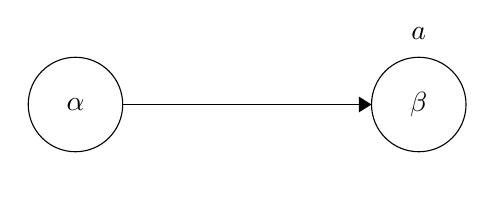
\begin{tikzpicture}[scale=0.2] 
\tikzstyle{every node}+=[inner sep=0pt] 
\draw [black] (22,-22.3) circle (3); 
\draw (22,-22.3) node {$\alpha$}; 
\draw [black] (43.8,-22.3) circle (3); 
\draw (43.8,-22.3) node {$\beta$}; 
\draw (22,-17.8) node {$\dia$}; 
\draw (43.8,-17.8) node {$a$}; 
\draw (43.8,-27.1) node {\sout{$\dia$}}; 
\draw (22,-27.1) node {\sout{$\diam{\dia}$}}; 
\draw [black] (25,-22.3) -- (40.8,-22.3); 
\fill [black] (40.8,-22.3) -- (40,-21.8) -- (40,-22.8); 
\end{tikzpicture} 
\end{center}


\section{Relazione Diretta}

\begin{tabular}{|c|c|c|}
\hline 
$\diam{\boa}\implies\boxx{\dia}$  & relazione diretta  & $\forhten{\alpha,\beta}{,\gamma:\:(\alpha R\beta\wedge\alpha R\gamma)}{\exists\delta:\,(\beta R\delta\wedge\gamma R\delta)}$\tabularnewline
\hline 
\end{tabular}

Ip) R è diretta

Ts) $\diam{\boa}\implies\boxx{\dia}$ 

Se l'antecedente è falso, il teorema è dimostrato. poniamoci quindi
nel caso:

$\veraw{\mu}{\alpha}{\diam{\boa}}$

avremo allora che:

$\exists\beta:\,\alpha R\beta\wedge\veraw{\mu}{\beta}{\boa}$

allora necessariamente si avrà che:

$\exists\delta:\,\beta R\delta\wedge\veraw{\mu}{\delta}a$

allora si avrà che:

$\veraw{\mu}{\beta}{\dia}$

prendiamo ora un qualsiasi mondo$\gamma$ tale che $\alpha R\gamma$,
poichè la relazione è diretta si avrà $\gamma R\delta$, e quindi:

$\veraw{\mu}{\gamma}{\dia}$

e allora possiamo osservare che vale:

$\veraw{\mu}{\alpha}{\boxx{\dia}}$

e la tesi è dimostrata

\begin{center} 
\begin{tikzpicture}[scale=0.2] 
\tikzstyle{every node}+=[inner sep=0pt] 
\draw [black] (17.1,-28) circle (3); 
\draw (17.1,-28) node {$\alpha$}; 
\draw [black] (33.1,-19.2) circle (3); 
\draw (33.1,-19.2) node {$\beta$}; 
\draw [black] (33.1,-38.3) circle (3); 
\draw (33.1,-38.3) node {$\gamma$}; 
\draw [black] (48,-28) circle (3); 
\draw (48,-28) node {$\delta$}; 
\draw (17.1,-23.7) node {$\diam{\boa}$}; 
\draw (33.1,-14.3) node {$\boa$}; 
\draw (48,-23.1) node {$a$}; 
\draw (33.1,-42.8) node {$\dia$}; 
\draw (17.1,-21.1) node {$\boxx{\dia}$}; 
\draw (33.1,-11.7) node {$\dia$}; 
\draw [black] (19.62,-29.62) -- (30.58,-36.68); 
\fill [black] (30.58,-36.68) -- (30.18,-35.82) -- (29.63,-36.66); 
\draw [black] (19.73,-26.55) -- (30.47,-20.65); 
\fill [black] (30.47,-20.65) -- (29.53,-20.59) -- (30.01,-21.47); 
\draw [black] (35.68,-20.73) -- (45.42,-26.47); 
\fill [black] (45.42,-26.47) -- (44.98,-25.64) -- (44.47,-26.5); 
\draw [black] (35.57,-36.59) -- (45.53,-29.71); 
\fill [black] (45.53,-29.71) -- (44.59,-29.75) -- (45.16,-30.57); 
\end{tikzpicture} 
\end{center}

Ip) $\diam{\boa}\implies\boxx{\dia}$ 

Ts) R è diretta

Supponiamo per assurdo R non diretta.

Consideriamo la funzione di valutazione:

$V(a)=\{\delta|\beta R\delta\}$

supponiamo che:

$\exists\alpha:\,\veraw{\alpha R\beta\wedge\mu}{\alpha}{\diam{\boa}}$

allora si avrà:

$\veraw{\mu}{\beta}{\boa}$

Prendiamo ora un qualsiasi mondo $\gamma$ tale che $\alpha R\gamma$,
e supponiamo che:

$\nexists\eta:\,\gamma R\eta$

Si avrà dunque che

$\nonveraw{\mu}{\gamma}{\dia}$

allora avremo che:

$\nonveraw{\mu}{\alpha}{\boxx{\dia}}$

che è assurdo, perchè contraddice la tesi. La tesi è allora valida.

\begin{center} 
\begin{tikzpicture}[scale=0.2] \tikzstyle{every node}+=[inner sep=0pt] 
\draw [black] (16.5,-26) circle (3); 
\draw (16.5,-26) node {$\alpha$}; 
\draw [black] (32.1,-15.3) circle (3); 
\draw (32.1,-15.3) node {$\beta$}; 
\draw [black] (46.9,-26) circle (3); 
\draw (46.9,-26) node {$\delta$}; 
\draw [black] (32.1,-37.6) circle (3); 
\draw (32.1,-37.6) node {$\gamma$}; 
\draw (16.5,-21.3) node {$\diam{\boa}$}; 
\draw (31.9,-10.5) node {$\boa$}; 
\draw (46.9,-21.3) node {$a$}; 
\draw (31.9,-32.8) node {\sout{$\dia$}}; 
\draw (16.5,-18.9) node {\sout{$\boxx{\dia}$}}; 
\draw [black] (18.97,-24.3) -- (29.63,-17); 
\fill [black] (29.63,-17) -- (28.68,-17.04) -- (29.25,-17.86); 
\draw [black] (34.53,-17.06) -- (44.47,-24.24); 
\fill [black] (44.47,-24.24) -- (44.11,-23.37) -- (43.53,-24.18); 
\draw [black] (18.91,-27.79) -- (29.69,-35.81); 
\fill [black] (29.69,-35.81) -- (29.35,-34.93) -- (28.75,-35.73); 
\end{tikzpicture} 
\end{center}
